\documentclass[12pt]{article}
\usepackage[utf8]{inputenc} % Required for inputting international characters
\usepackage[T1]{fontenc} % Output font encoding for international characters

\usepackage{mathpazo} % Palatino font

\setcounter{tocdepth}{5} %to make it appears in TOC
\setcounter{secnumdepth}{5} %to make it numbered

%image preamble
\usepackage{graphicx}
\usepackage{float}


\usepackage{hyperref}
\hypersetup{
    colorlinks=true,
    linkcolor=blue,
    filecolor=magenta,      
    urlcolor=cyan,
}

%list preamble
%\renewcommand{labelitemi}{$\bullet$}
%\renewcommand{labelitemii}{$\circ$}

%starting the document
\begin{document}

\begin{titlepage} % Suppresses displaying the page number on the title page and the subsequent page counts as page 1
	\newcommand{\HRule}{\rule{\linewidth}{0.5mm}} % Defines a new command for horizontal lines, change thickness here
	
	\center % Centre everything on the page
	
	%------------------------------------------------
	%	Headings
	%------------------------------------------------
	
	\textsc{\LARGE Netaji Subhas University of Technology}\\[1.5cm] % Main heading such as the name of your university/college
	
	\textsc{\Large Operating System Case Study}\\[0.5cm] % Major heading such as course name
	
	\textsc{\large CECSC09}\\[0.5cm] % Minor heading such as course title
	
	%------------------------------------------------
	%	Title
	%------------------------------------------------
	
	\HRule\\[0.4cm]
	
	{\huge\bfseries Lynx OS : A Case Study}\\[0.4cm] % Title of your document
	
	\HRule\\[1.5cm]
	
	%------------------------------------------------
	%	Author(s)
	%------------------------------------------------
	
\begin{minipage}{0.4\textwidth}
\begin{flushleft} \large
\emph{Authors:}\\
Daksh Gupta \\ \textit(2019UCO1669)\\Aansh Sardana\\ \textit(2019UCO1672)% Your name
\end{flushleft}
\end{minipage}
~
\begin{minipage}{0.4\textwidth}
\begin{flushright} \large
\emph{Supervisor:} \\
Ms. Savita Yadav\\Asst. Professor\\Dept. of CSE\\NSUT % Supervisor's Name
\end{flushright}
\end{minipage}\\[1cm]
	
	% If you don't want a supervisor, uncomment the two lines below and comment the code above
	%{\large\textit{Author}}\\
	%John \textsc{Smith} % Your name
	
	%------------------------------------------------
	%	Date
	%------------------------------------------------
	
	\vfill\vfill\vfill % Position the date 3/4 down the remaining page
	
	{\large Made Using LaTeX} % Date, change the \today to a set date if you want to be precise
	
	%------------------------------------------------
	%	Logo
	%------------------------------------------------
	
	%\vfill\vfill
	%\includegraphics[width=0.2\textwidth]{placeholder.jpg}\\[1cm] % Include a department/university logo - this will require the graphicx package
	 
	%----------------------------------------------------------------------------------------
	
	\vfill % Push the date up 1/4 of the remaining page
	
\end{titlepage}
\tableofcontents
\cleardoublepage

\section{Introduction}\label{sec:intro}
\subsection{What is an Operating System?}
An operating system, a computer program that can support a computer’s basic functions,
and can provide services to other programs that can run on a computer. The computer can be any
system like a home desktop, a mobile device, or an embedded hardware system that has
functionalities where a user can manipulate it and be able to use the services that operating
system provides. The user will have needs or wants that a computer will be able to handle,
control, or direct through the services, or in other words, applications or programs, that the user
can run on the computer. An operating system (OS) helps to write, maintain, and use these
applications faster and simpler than having to backtrack through lines of code that a developer
has written for the application. An example of this, will be the web browser in a desktop. The
web browser is an application that is running within the operating system’s environment.
Most operating systems usually allow for multiple applications to run at the same time.
When more than one application is running at the same time as another, this is called multitasking. A unit within the operating system, called the scheduler, decides what programs to run,
when that specific program should run, and in a way, provides the user to see that multiple
programs are running at the same time. These programs seem to run at the same time, but is an
“illusion of simultaneous execution by rapidly switching between each program.”
How an operating system is distinct from another OS, since there are multiple types, is by
how the scheduler decides on which program gets to run first and so on. The scheduler in the
operating system is what distinguishes a variant OS from one another. For example, the ‘UNIX
OS will make sure that each program gets a fair share of the CPU processing time, whereas the
Microsoft Windows OS tries to make sure that the computer stays responsive for its user.’ Even
though both examples are their own operating systems in their own functionality, both share the
reason that they make sure the scheduler runs only for the OS that they are programmed for. 

\subsection{Who is Lynux Works and what is Lynx OS?}
LynxOS and LynxOS-178 are embedded real time operating systems marketed by
LynuxWorks of San José, California. LynxOS, the first real time operating system
developed by LynuxWorks, was introduced in 1988. LynxOS-178 was built on the
LynxOS framework but was developed for systems seeking to meet the DO-178B
standards.\\
 It is based off the UNIX operating system,
which is also based off Linux, and it confirms to the POSIX set of standards and makes sure to
use the most concise of the embedded kernel footprint that is found most embedded systems
today. POSIX is short for ‘Portable Operating System Interface for uni-X’ and are standards that
were developed by the Institute of Electrical and Electronic Engineers (IEEE) to ease “the task of
developing programs where the developer only has to write a program once to run all POSIXcompliant systems.” 6 LynxOS uses POSIX-compliant APIs (Application Programming
Interface) which provide symmetric multi-processing support so that the operating system can
take full control of any multi-core processors.\\
Not only does LynxOS have a host of different APIs that allow for better control of the
multi-core processors, but it does have an array of tools, debuggers, and cross-development
support for multiple systems. The support alone for these multiple systems allows for I/O
technology support, as well as to enable any state-of-the-art security features that may exist
today. An application in LynxOS well also be able to rely on the operating system’s real-time
determinism feature. It is considered a foundational feature were a “predictable response is
ensured even in the presence of heavy I/O as a result of the kernel’s unique and highly optimized
threading model.”\\
\subsection{Where is Lynx OS found?}
LynxOS can be found in a variety of modern application systems, including trades such
as military, aeronautical, medical, and industry. The operating system even helps businesses that
are based in office automation as they “benefit from security and networking
improvements”
that are found in next-gen LynxOS architectures. The one industry that LynxOS can be found in the most is that of aeronautical and aerospace application design. In avionics, the
operating system must be able to meet the DO-178 standards which were set by the Federal
Aviation Administration (FAA). The DO-178 standards is a straightforward way of being able to
certify developed aviation software as being safe for avionic use. Any additional information
regarding to the DO-178 standards can be found under Title 14: Aeronautics and Space of the
Code of Federal Regulations (CFR), Part 21, Subpart O. Since LynxOS has the DO-178
certification
, as well as military certifications, several systems that have been developed in
LynxOS include \cite{ref:six}:

\begin{itemize}
	\item Airbus A380 Superjumbo Flight Test and Simulation
	\item Boeing 777 Cabin Services System
	\item Common ARTS Air Traffic Control Systems
	\item NASA’s SLR2000 Satellite Ranging System
	\item Raytheon MK 57 Launching System DD(X)
\end{itemize}

As noted, most of these application systems were developed in the security of human life. As
explained before, a Real-Time Operating System must be able to act as needed before a deadline.
If there is a miscalculated step, or an improper performance spike, there will be a risk of human
life casualties.

\cleardoublepage

% Second section
\section{Embedded Systems}\label{sec:embedded}

The first question that is needed to be answered is that what is an embedded system? The following systems can be called an embedded system:

\begin{itemize}

	\item Which performs its duty completely or partially, without human’s intervention?	
	\item Which interacts with physical environment, like driving a motor?
	\item Which is built to perform only specific tasks but with high efficiency?
	
\end{itemize}

There are different definitions for embedded systems but in summary, an embedded system is a microprocessor that is used as a component to do
a specific task in another system like cell phones, household appliance and even a keypad for entering a password.
The other main question is that, Are embedded systems common? To answer this question briefly, it’s enough to say according to \cite{ref:embed}\\

Embedded systems, as is shown in Figure \ref{fig:embedarch}, generally include a control loop where a microcontroller reads signals from sensors that are attached
to some equipment out in the real world (IRL). Based on those sensor readings, the microcontroller calculates some changes which it wants to
make IRL to control the equipment. The equipment responds to these changing signals, which changes the sensor readings.

\begin{figure}[H]
	\centering
	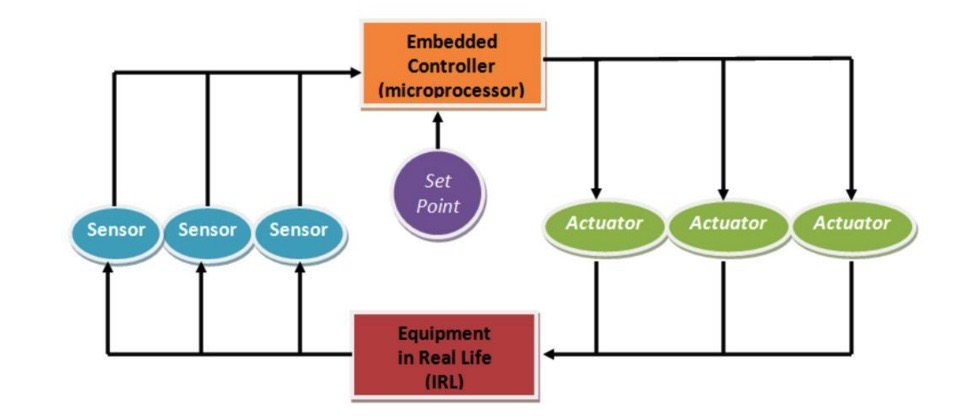
\includegraphics[width=13cm,height=10cm,keepaspectratio]{/Users/daksh_mac/Desktop/embed.jpeg}
	\caption[About embedded system]{Embedded System Architecture}
	\label{fig:embedarch}	
\end{figure}

\subsection{Embedded System History}
One of the first embedded modern systems was Apollo Guidance Computer, developed by Charles Stark Draper at the MIT Instrumentation
Laboratory. The automatics D-17 embedded system guidance computer for the Minuteman missile system was, released in 1961. When the
Minuteman II produced in 1966, the D-17 was replaced with a new system that was the first high-volume use of integrated circuits. In the 1960s,
embedded systems’ price has come down and processing power and functionality have been raised. For example, Intel4004, the first
microprocessor, was designed for calculators and other small systems but still needed many external memory and support chips.\\
In 1978, a "standard" released for programmable microcontrollers by National Engineering Manufacturers Association which included almost
any computer-based controllers, such as single board computers, event-based, and numerical controllers. In the middle of 1980s, most of the
common previously external system components had been integrated into the same chip as the processor. The integration of microcontrollers has
further increased the applications for which embedded systems are used into areas where traditionally a computer would not have been
considered.
\subsection{Embedded System Categories}
According to \cite{ref:embedcat}, embedded systems can be divided into 4 general categories: general computing, communication and networking, signal
processing and control system. These types are explained in the following.

\begin{itemize}

	\item General Computing: In this type of embedded systems, applications are similar to desktop computing but are in an embedded package.
Some examples of this type are Video games, automatic tellers, wearable computers, set-top boxes and etc.	
	\item Communications: These types of embedded systems are used for switching and also information transition, so cell phone system and
internet are some examples of this type of embedded systems. They can be found in every where now a days and are very common
	\item Signal processing: Embedded systems which are in signal processing category are used when computations involve large data streams.
Some examples of these systems are radar, sonar, video and audio compressions and etc. these types of embedded systems have more
special usage and cannot be seen everywhere. 
	\item Control: Embedded systems which are used for real-time feedback control, place in control category. In this type having a proper
RTOS can be very useful to improve the system’s performance. Nuclear power, medical processes and flight control are some cases
that use this type of embedded systems.
	
\end{itemize}

\subsection{Embedded Systems Factors}
Embedded systems are distinguished from many factors like cost, safety, real time critical, reliability, weight, size and some other factors.
Embedded systems should have maximum performance with minimum weight and size. They also should be efficient, to explain more, they are
designed to do repeated functions for a long time, so they shouldn’t require to be serviced. Embedded systems should really be real time \cite{ref:eight}.
Some embedded systems are used in equipments which are in contact with human’s life so they should answer right without any delay. In
summary, they must be efficient from every opinion, run-time efficient, energy efficient, weight efficient, size efficient, cost efficient, code-size
efficient, etc . The focus of this paper is on real time issue. Operating systems play a significant role in real time systems.


\subsubsection{RTOS}
A real-time operating system (RTOS) schedules tasks in a way to be performed according to priorities, so the execution can be reliable. Figure \ref{fig:kernel}
illustrates its kernel functions. The distinctive feature of a RTOS from other types of operating systems is that, it is typically implemented as a
kernel. In RTOS the kernel is a layer of abstraction between the hardware layer and the applications layer where the tasks are running.

\begin{figure}[H]
	\centering
	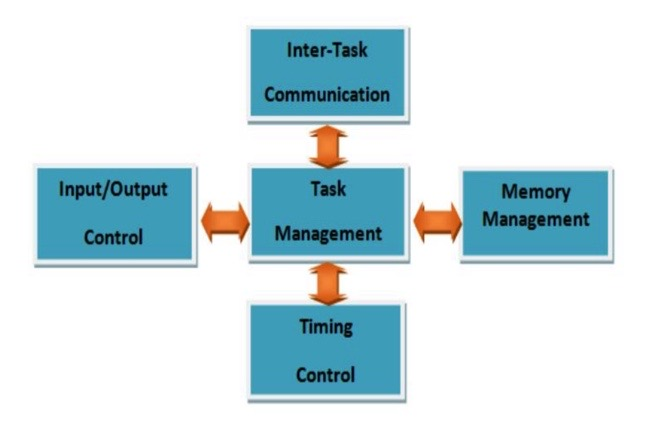
\includegraphics[width=13cm,height=10cm,keepaspectratio]{/Users/daksh_mac/Desktop/kernel.jpeg}
	\caption[About kernel functions]{RTOS Kernel Functions}
	\label{fig:kernel}	
\end{figure}

Real time systems are used in time- critical applications such as fight control system, medical equipment, etc. .Therefore a real-time system must
complete its work and deliver its service in a specific deadline. A RTOS helps a lot in creation of a real-time system, but doesn’t guarantee that
the final product is real-time.

\paragraph{Lynx OS}

It is a pre-emptive OS, so it can be used in reasonable situations and also it guarantees that processes which are time-critical will terminate
instantly that is a good property for real-time embedded systems. This OS can be formed to be multi-threaded, that is a positive point in
networked systems.\\
The use of memory management unit (MMU) is required for LynxOS and this matter is good because o†f safety but is not a positive point for
flexibility. It uses the MMU to address virtual memory although it makes the system slower. LynxOS is self-hosting, which means that the user
program can develop by using the OS as a platform. This OS uses multiple address spaces, which makes it slower because of doing a lot of
context switching, but it is done to be safety \cite{ref:per}.


\section{Design Goals and Approach}\label{sec:design}

\subsection{Design Goals of Lynx OS}
Four design goals outlined by Vik Sohal, LynuxWorks Technical Sales, are summarized
below:

\begin{itemize}

	\item The operating system kernel had to be preemptive and reentrant. This was
important so time-critical tasks will execute promptly.	
	\item The kernel supports multithreading. User programs, device drivers and other
kernel services can create their own tasks that are called kernel threads. More
detail on kernel threads including scheduling and advantages are provided later in
this paper. 
	\item LynxOS uses a processor's page memory management unit (MMU) to provide
each instance of a user process its own protected logical address space. The MMU
also protects the kernel by placing it in a separate address space.
	\item LynxOS utilizes Unix and POSIX APIs, allowing:
		\begin{itemize}
			\item[$\circ$] a variety of Unix programs to be ported to LynxOS and 
			\item[$\circ$] offering a shallow learning curve for those programmers already familiar
with the interface 
		\end{itemize}
	
\end{itemize}

\subsection{Lynx OS Approach}

In order to achieve the first two goals (prompt execution and multithreading),
LynxWorks developed and patented techniques known as kernel threads and priority
tracking. To address goal three (memory protection), LynuxWorks utilizes the
processor's page memory management unit (MMU). For the last noted goal (portability
and less steep learning curve), LynxOS utilizes Unix and POSIX APIs. Each of these
approaches will be discussed in further sections. 

\cleardoublepage


\section{Structural Overview}\label{sec:architecture}
\subsection{Architecture of Lynx OS}
First, LynxOS runs on a microkernel architecture, also known as its own “separation
kernel” where it can combine secure and real-time components using varying partitions within
the system design. A microkernel is a minimal OS kernel where it is less prone to errors, system
services are easier to implement at user-level servers between the connections of multiple
applications, and has a better protection between individual components in the system \cite{ref:arch}

\begin{figure}[H]
	\centering
	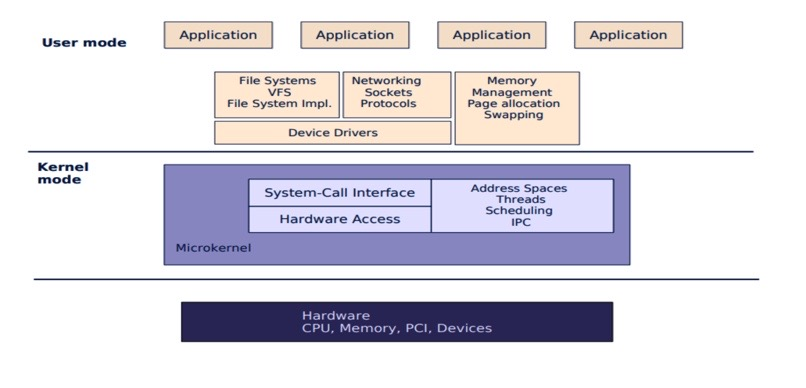
\includegraphics[width=14cm,height=10cm,keepaspectratio]{/Users/daksh_mac/Desktop/arch1.jpeg}
	\caption[About arch]{Basic Microkernel Model}
	\label{fig:arch1}	
\end{figure}


A microkernel based operating system also has the safe possibility that if one component decides
to crash, or terminate on its own because of a failure, it doesn’t necessarily crash the entire
system. The component that is running on a separate partition of the system, will only crash
within that partition without affecting the other partitions controlling the other components or
applications. As noted, applications and system services exist within partitions, where the
hardware components exist in their own level.

\begin{figure}[H]
	\centering
	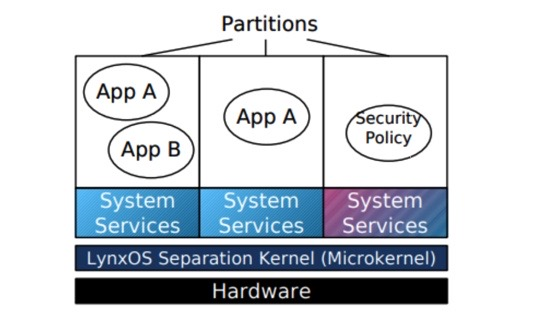
\includegraphics[width=13cm,height=10cm,keepaspectratio]{/Users/daksh_mac/Desktop/arch2.jpeg}
	\caption[About arch]{Lynx OS Partition System}
	\label{fig:arch1}	
\end{figure}

\subsection{Component Structure of LynxOS}
One of the operating systems that Lynx Software Technologies prides on of course its
LynxOS-178 Certified RTOS which is the operating system of choice for some developers when
designing applications and systems for aerospace and aeronautical use. Remember that, because
the operating system is DO-178 certified, it means that the operating system passed all tests
regarding that the OS was fit for use and was able to pass all safety measurements that the FAA
takes care of. Within the LynxOS package, there exist components that serve to protect the
controller and the system that is running on LynxOS. Most of the important safety features of the
operating system exist in the ARINC 653 Services package. This a multitude of many services
that make sure to check on services such as partition management, process management, time
management, and of course interpartition communication which is responsible for any
communication to exist between the services that exist in the multiple partitions of the system.\\

Since LynxOS is a microkernel based operating system, and as noted before, this is
known as the separation kernel that exists on the bounds of software and hardware, a key
component that really makes up for this structure is the ARINC 653 Health Monitoring
component. This component is important because it is a component that lets the OS know that an
error has occurred and is predicting a fault within the system itself. The component is invoked by
either the service application, the OS, or even the hardware that is becoming faulty as the alert is
being sent out. Since LynxOS wants to achieve complete system security, it uses “Virtual
Machine (VM) brick-wall partitions of time, memory and resources.” Each of these partitions
in a way acts like a stand-alone version of the operating system on its own. Any system events
that occur in the OS, in either one of the partitions cannot share any resources or interfere with
other system events in any of the other partitions. The only partition that can be interfered with is
Virtual Machine Zero (VM0), which handles system administrative services within the root of
the POSIX system services unit.

\begin{figure}[H]
	\centering
	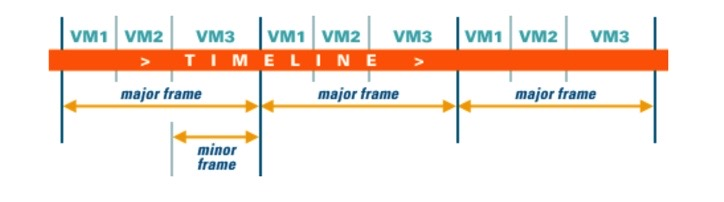
\includegraphics[width=14cm,height=10cm,keepaspectratio]{/Users/daksh_mac/Desktop/arch3.jpeg}
	\caption[About arch]{ARINC 653 Health Monitoring Component}
	\label{fig:arch1}	
\end{figure}

Another special component of LynxOS is the CPU Support Package (CSP) which
contains all the processor routines, which includes the MMU, the floating point, and the
processor exception handlers. These routines are all linked to the LynxOS-178 microkernel. This
package contains multilevel system setup routines that apply to hardware, system software, and
the application software within the system that is being designed. For example, the above
mentioned ARINC 653 Health Monitor exists in the application software level, but stays within
the first partition. This monitor is then linked to the system software’s partitioning kernel that
makes sure that all connections are secured and functioning. From here, the connections are then linked to the CSP, board support package, or to any of the other middleman packages that exist
between the system software and hardware levels. After passing through these packages, the link
is made once more to either the microprocessor, any hardware components, the PCI controller, or
any optional hardware that isn’t connected to one of the main pieces of equipment. This structure
maintains that all partitions are separated from one another, so that LynxOS can run on them
separately, but still makes sure that all connections are made within the computing system.

\begin{figure}[H]
	\centering
	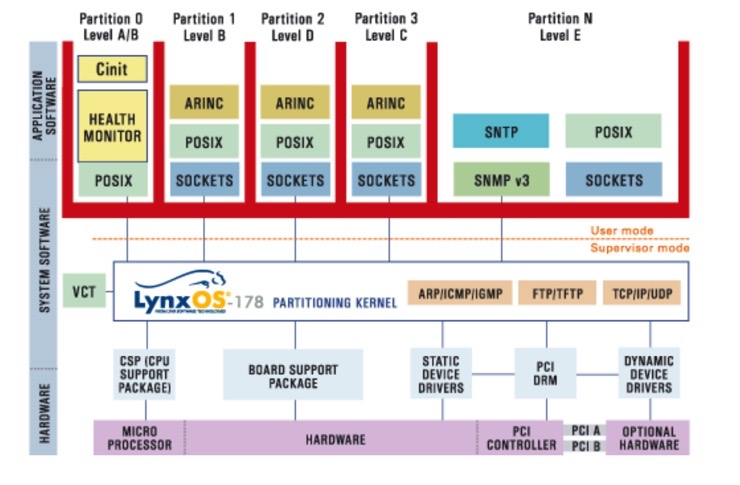
\includegraphics[width=14.5cm,height=10cm,keepaspectratio]{/Users/daksh_mac/Desktop/arch4.jpeg}
	\caption[About arch]{LynxOS Structure Model}
	\label{fig:arch1}	
\end{figure}
\cleardoublepage

\section{Process and Thread Organization}\label{sec:procThread}

\subsection{General Definitions}

\begin{itemize}

	\item \emph{Process}: A process is basically a program in execution. The execution of a process must progress in a sequential fashion.
	
	\item \emph{Thread}: A process is basically a program in execution. The execution of a process must progress in a sequential fashion.
	
	\item \emph{Process Control Block}:  The process control block stores the register content also known as execution content of the processor when it was blocked from running like process state, program counter, context, CPU registers, CPU-scheduling information,  Memory-management information, Accounting information,  I/O status information. 
	
	\item \emph{Process Scheduling}: The process scheduling is the activity of the process manager that handles the removal of the running process from the CPU and the selection of another process on the basis of a particular strategy.
Process scheduling is an essential part of a Multiprogramming operating systems. Such operating systems allow more than one process to be loaded into the executable memory at a time and the loaded process shares the CPU using time multiplexing.

       \item \emph{Type of Queues}:
       		\begin{itemize}
			\item \emph{Ready Queue}: This queue keeps all the processes in the system.
			\item \emph{Job Queue}: his queue keeps a set of all processes residing in main memory, ready and waiting to execute. A new process is always put in this queue.
			\item \emph{Device Queue}: The processes which are blocked due to unavailability of an I/O device constitute this queue.
		\end{itemize}
 	
\end{itemize}

\begin{figure}[H]
	\centering
	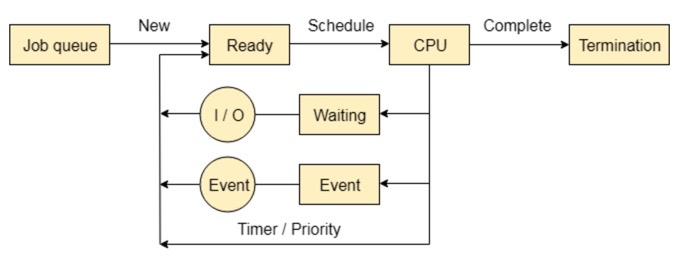
\includegraphics[width=14.5cm,height=10cm,keepaspectratio]{/Users/daksh_mac/Desktop/queue.jpeg}
	\caption[About queues]{Functioning of Queues}
	\label{fig:queue}	
\end{figure}

\begin{itemize}
	\item \emph{Context Switching}: A context switch is the mechanism to store and restore the state or context of a CPU in Process Control block so that a process execution can be resumed from the same point at a later time. Using this technique, a context switcher enables multiple processes to share a single CPU. Context switching is an essential part of a multitasking operating system features.
	
	
	\item \emph{Interprocess communication}: Inter Process Communication (IPC) refers to a mechanism, where the operating systems allow various processes to communicate with each other. This involves synchronizing their actions and managing shared data.
	
	\item \emph{Multithreading}: In computer architecture, multithreading is the ability of a central processing unit (CPU) (or a single core in a multi-core processor) to provide multiple threads of execution concurrently, supported by the operating system.
	
	\item \emph{Multiprocessing}: Multiprocessing is the use of two or more central processing units (CPUs) within a single computer system.[1][2] The term also refers to the ability of a system to support more than one processor or the ability to allocate tasks between them
	
\end{itemize}

\cleardoublepage

\subsection{Issues Associated With Task Schedueling }

Before we go on describing how processes are actually scheduled , we need to understand the problems associated with it's scheduling and execution.

\subsubsection{Priority Inversion}

A primary issue with task scheduling is known as priority inversion. As shown in Figure
\ref{fig:inversion} ,priorty inversion is the situation where a high priority task is running but is preempted
by an asynchronous interrupting device for a lower priority task. Priority inversion can
also be seen as hardware interrupts or kernel processes that steal cycles from high priority
tasks and degrade an application’s ability to meet real-time deadlines. In general, routine
processing in most systems can lead to problems where high priority processes find
themselves constantly interrupted by hardware events.\\\\
Asynchronous interrupting devices are most any unit that generates a requested or
unsolicited signal that supplies the system with information. Examples of these include,
but are not limited to: network interfaces, console displays, keyboards, disk controllers
and external timers.\\

\begin{figure}[H]
	\centering
	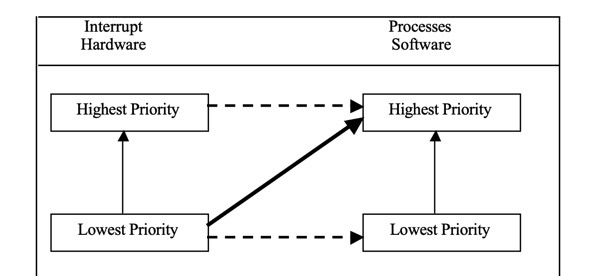
\includegraphics[width=10cm,height=10cm,keepaspectratio]{/Users/daksh_mac/Desktop/inversion.jpeg}
	\caption[About Priority Inversion]{In the above scenario, data is being requested for low priority process. Without kernel sthreads, hardware interrupts would trigger when the data becomes available. Since
hardware interrupts run at higher priority than processes, the interrupt will pull resources
from the high priority time-critical process.}
	\label{fig:inversion}	
\end{figure}

\cleardoublepage

\subsection{Process Management and Schedueling}

The basic LynxOS scheduling entity is the thread and LynxOS scheduling is preemptive,
reentrant and based on one of three selected scheduling policies: 

\begin{itemize}
	\item \emph{First-In-First-Out}
	
	
	\item \emph{Round Robin}
	
	\item \emph{Priority Based Quantum} -  Lynx proprietary policy that is similar to round robin
but includes a configurable time quantum for each priority level.

\end{itemize}	

In order to understand how LynuxWorks deals with priority inversion, it is important to
understand that LynxOS is \emph{POSIX-conformant} and that the basic LynxOS scheduling
entity is the thread. This means that threads are the running entities of LynxOS. 

\subsubsection{POSIX in LynxOS}

\paragraph{What is POSIX?} 
POSIX is an abbreviation for Portable Operating System Interface. As briefly explained above, POSIX is the name for a collection of standards that are required to maintain compatibility between operating systems.

\paragraph{What Does Being POSIX-Compliant Mean?} 
The term “POSIX-compliant” means that an operating system meets all the POSIX criteria


\paragraph{Involvement of POSIX in Lynx OS} 

POSIX assumes that each process in a system resides in a different address space.  In order to do this, LynxOS-178 uses the Memory Management Unit (MMU) of the processor to physically isolate the processes from each other so that they cannot access each other’s memory; this makes systems more robust by preventing one process from reaching over and accidentally (or illicitly) accessing the address space of another process.\\
On LynxOS-178 and other POSIX operating systems, a user application can only address data in an address range known as “user space”.  The remaining portion of the address space is called “kernel space”. 




\subsubsection{LynxOS Scheduling}
\emph{LynxOS 3.0.1 supports a single scheduling policy, fixed priority preemption with 256 priority levels.}\cite{ref:nine} \\\\

In preemptive
scheduling, a process that is currently running can be interrupted if a higher priority process
comes into the schedulers view. The current running process will be paused and will allowed to
be finished until the new process has finished. Adding priority to this means that if a process has
a higher priority than a lower priority item that is currently running, the lower priority item will
be paused and allows the higher priority item to cut in front of the line.\\
LynxOS' scheduling was
designed to be preemptive and reentrant, as well as being based on scheduling algorithms such as
First-In, First-Out and Round Robin. This allows the operating system to set true task priorities
and task preemption into the kernel. The operating system even goes beyond this by making sure
to execute any extended and asynchronous interrupts that are being processed at any task priority
levels. Even if there are any preemption delays or blocking times that can be caused by a fault in
the kernel, these can be used in conjunction with other task execution times so that single tasks
can reach their deadlines on time and without process faults

\begin{figure}[H]
	\centering
	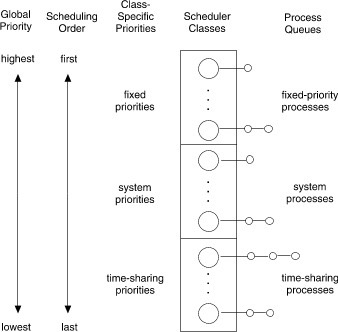
\includegraphics[width=13cm,height=10cm,keepaspectratio]{/Users/daksh_mac/Desktop/posixSch.jpeg}
	\caption[About scheduling]{Scheduling in Lynx OS}
	\label{fig:sch}	
\end{figure}

LynxOS is divided into 256
priorities. These priorities are further subdivided to make 512 priorities. This includes
the original 256 plus a half step above each of the original priorities. Kernel threads
begin their existence with a very low priority (usually 0) as created by a driver. When a
user thread opens the device, the kernel thread promotes its own priority and "inherits"
the priority of the user thread opening the device. If another user thread of higher priority
opens the device, the kernel thread bumps its priority up to match the other thread; when
the I/O is complete the kernel thread returns to the next pending thread's priority level, or
to its starting level. With the changes, we can see that the kernel thread tracks or follows
the priority of device that calls it. The following example \cite{ref:seven} demonstrates how the priority
of the kernel thread tracks the user threads that opened the device and cause the kernel
thread to be created.


\begin{table}[H]
%\centering

\label{tab:schEx}
\caption[scheduling example]{Scheduling example is Lynx OS}

\noindent\makebox[\textwidth]{
\begin{tabular}{c|c}
\bfseries{Kernel Thread initial creation} & \bfseries{Kernel Thread Priority} \\ \hline
User thread (priority 10) opens device - kernel thread promotion & 10 \\
User thread2 (priority 20) opens device – kernel thread promotion & 20 \\
User thread2 completes – kernel thread demotion & 10 \\
User thread3 (priority 60) opens device – kernel thread promotion &  60 \\
User thread4 (priority 30) opens device – kernel thread remains unchanged & 60 \\
User thread3 completes – kernel thread demotion & 30 \\
User thread4 completes – kernel thread demotion & 10  \\
User thread2 completed – kernel thread demotion & 0  \\
\end{tabular}
}

\end{table}


\subsubsection{LynxOS Interrupt Handling System}

The LynxOS has an intriguing interrupt system that handles interruption unlike any other
RTOS. During the date of the published work for where this is being researched from, the
AAUGN states that “most operating systems simply execute interrupt processing to completion,
allowing it to be preempted only by higher priority interrupts.” Since it is possible for a
computer to be connected to a network, have access to a mass storage device, or having to handle
a user interface, the computer can receive multiple hardware interruptions from various sources
at the same time. As the scheduler is running, this would put strain on the CPU, as it would steal
time from the tasks that would really need the CPU. But LynxOS does come to the rescue as it
solves this problem by executing a bulk of the interrupting services at the task priority level by
using dedicated kernel threads for these processes.\\

By the LynxOS approach, the driver's interrupt handler does a minimum of work and
signals the kernel thread that interrupt-related data is available. LynxOS then treats these
threads like normal user threads, with software rather than interrupt priorities. If LynxOS
implemented kernel threads by themselves, the issue of \emph{priority inversion} would still
exist. As shown in Figure \ref{fig:ptrack}, by incorporating a technique known as \emph{priority tracking},
kernel threads can process interrupts but, at the same time, will be scheduled along with
user threads based on an “appropriate” thread priority. \\

The interrupt thread priority is based on the
highest priority task that has access to the device that is generating the interruption. Once the
task is located, any interruptions are re-engaged by the kernel thread. This puts a deadline bound
on the amount of time a high priority task can be delayed because of the interruptions. With this,
a system can be created to be predictable even when in the face of unpredictable interruptions
that can be caused in a very high, and stressful environment.

\begin{figure}[H]
	\centering
	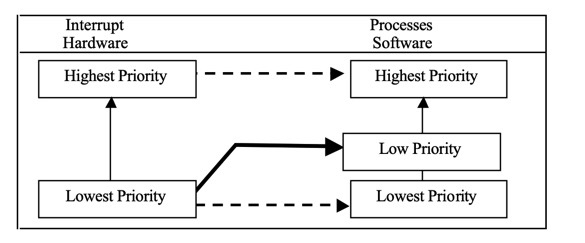
\includegraphics[width=14cm,height=10cm,keepaspectratio]{/Users/daksh_mac/Desktop/ptracking.jpeg}
	\caption[About Priority Tracking]{In the above scenario, data is again being requested for a low priority process. With
kernel threads and priority tracking, the device is opened and a kernel thread is created
and scheduled with a priority that is consistent with the requesting process. With this, the
kernel thread will be processed at an appropriate time as determined by the scheduling
rules without pulling resources from the higher priority time-critical process.}
	\label{fig:ptrack}	
\end{figure}

\subsection{Interprocess Communication and Process Synchronization}

Interprocess Communication mechanism allow arbitrary processes to exchange data and synchronize execution. 

Lynx OS uses Unix-like System-V IPC package for communication. The three forms of communication under this package are described in these subsections \cite{ref:twelve}.

\begin{itemize}
	\item Messages allow processes to send formatted data streams to arbitrary processes.
	
	
	\item Semaphores allow processes to synchronize execution.
		
	\item Shared memory allows processes to share parts of their virtual address space.

\end{itemize}	


\subsubsection{Permissions}

Messages, semaphores, and shared memory have read and write permissions (but no execute permission) for the owner, group, and others the same as ordinary files. Like files, the creating process identifies the default owner. Unlike files, the creator can assign ownership of the facility to another user; it can also revoke an ownership assignment.

\subsubsection{System V Messages}

Before a process can send or receive a message, the queue must be initialized through the \emph{msgget(2)} function. The owner or creator of a queue can change its ownership or permissions using  \emph{msgctl(2)}. Also, any process with permission to do so can use \emph{msgctl(2)} for control operations.

IPC messaging lets processes send and receive messages, and queue messages for processing in an arbitrary order. Unlike the file byte-stream data flow of pipes, each IPC message has an explicit length.

Messages can be assigned a specific type. Because of this, a server process can direct message traffic between clients on its queue by using the client process PID as the message type. For single-message transactions, multiple server processes can work in parallel on transactions sent to a shared message queue.

Operations to send and receive messages are performed by the \emph{msgsnd(2)} and \emph{msgrcv(2) }functions, respectively. When a message is sent, its text is copied to the message queue. The \emph{msgsnd(2)} and \emph{msgrcv(2)} functions can be performed as either blocking or non-blocking operations. A blocked message operation remains suspended until one of the following three conditions occurs:

\begin{itemize}
	\item The call succeeds.
	
	
	\item The process receives a signal.	
		
	\item The queue is removed

\end{itemize}	


\subsubsection{System V Semaphores}

Semaphores let processes query or alter status information. They are often used to monitor and control the availability of system resources such as shared memory segments. Semaphores can be operated on as individual units or as elements in a set.

Because System V IPC semaphores can be in a large array, they are extremely heavy weight. Much lighter weight semaphores are available in the threads library . Also, POSIX semaphores are the most current implementation of System V semaphores . Threads library semaphores must be used with mapped memory.

A semaphore set consists of a control structure and an array of individual semaphores. A set of semaphores can contain up to 25 elements. The semaphore set must be initialized using \emph{semget(2)}. The semaphore creator can change its ownership or permissions using semctl(2). Any process with permission can use \emph{semctl(2)} to do control operations.

Semaphore operations are performed by the \emph{semop(2)} function. This function takes a pointer to an array of semaphore operation structures. Each structure in the array contains data about an operation to perform on a semaphore. Any process with read permission can test whether a semaphore has a zero value. Operations to increment or decrement a semaphore require write permission.

When an operation fails, none of the semaphores is altered. The process blocks and remains blocked until:

\begin{itemize}
	\item The semaphore operations can all finish, so the call succeeds
	
	
	\item The process receives a signal
		
	\item The semaphore set is removed

\end{itemize}	

Only one process at a time can update a semaphore. Simultaneous requests by different processes are performed in an arbitrary order. When an array of operations is given by a \emph{semop(2)} call, no updates are done until all operations on the array can finish successfully.
If a process with exclusive use of a semaphore terminates abnormally and fails to undo the operation or free the semaphore, the semaphore stays locked in memory in the state the process left it. To prevent this, the $SEM\_UNDO $control flag makes \emph{semop(2)} allocate an undo structure for each semaphore operation, which contains the operation that returns the semaphore to its previous state. If the process dies, the system applies the operations in the undo structures. This prevents an aborted process from leaving a semaphore set in an inconsistent state.
If processes share access to a resource controlled by a semaphore, operations on the semaphore should not be made with $SEM\_UNDO$ in effect. If the process that currently has control of the resource terminates abnormally, the resource is presumed to be inconsistent. Another process must be able to recognize this to restore the resource to a consistent state.


\subsubsection{System V Shared Memory}

In the Lynx OS operating system, the most efficient way to implement shared memory applications is to rely on the \emph{mmap} function and on the system's native virtual memory facility. 
Lynx OS also supports System V shared memory, which is a less efficient way to let multiple processes attach a segment of physical memory to their virtual address spaces. When write access is allowed for more than one process, an outside protocol or mechanism such as a semaphore can be used to prevent inconsistencies and collisions.

A process creates a shared memory segment using \emph{shmget(2)}. This call is also used to get the ID of an existing shared segment. The creating process sets the permissions and the size in bytes for the segment.

The original owner of a shared memory segment can assign ownership to another user with \emph{shmctl(2)}. It can also revoke this assignment. Other processes with proper permission can perform various control functions on the shared memory segment using \emph{shmctl(2)}.

Once created, a shared segment can be attached to a process address space using \emph{shmat(2)}. It can be detached using \emph{shmdt(2)}. The attaching process must have the appropriate permissions for \emph{shmat(2)}. Once attached, the process can read or write to the segment, as allowed by the permission requested in the attach operation. A shared segment can be attached multiple times by the same process.

A shared memory segment is described by a control structure with a unique ID that points to an area of physical memory. The identifier of the segment is called the \emph{shmid}. The structure definition for the shared memory segment control structure can be found in $<sys/shm.h>$

\subsection{Deadlock Handling in Lynx OS}
Sharing and allocating system resources between running and new processes is an operating system task. In a multiprocessing environment, allocation of resources can become a point of conflict. Such conflict may lead the system into a state known as \emph{deadlock}. The scope of the topic is to identify the conditions for deadlocks, distinguish the different circumstances that lead to this undesirable state, and identify the methods for detection, prevention, and recovery.

\subsubsection{Deadlock Avoidance}

The most common error causing deadlock in RTOS is self deadlock or recursive deadlock: a thread tries to acquire a lock it is already holding. Recursive deadlock is very easy to program by mistake.

For example, if a code monitor has every module function grabbing the mutex lock for the duration of the call, then any call between the functions within the module protected by the mutex lock immediately deadlocks. If a function calls some code outside the module which, through some circuitous path, calls back into any method protected by the same mutex lock, then it will deadlock too.

The solution for this kind of deadlock is to avoid calling functions outside the module when you don't know whether they will call back into the module without reestablishing invariants and dropping all module locks before making the call. Of course, after the call completes and the locks are reacquired, the state must be verified to be sure the intended operation is still valid.

An example of another kind of deadlock is when two threads, thread 1 and thread 2, each acquires a mutex lock, A and B, respectively. Suppose that thread 1 tries to acquire mutex lock B and thread 2 tries to acquire mutex lock A. Thread 1 cannot proceed and it is blocked waiting for mutex lock B. Thread 2 cannot proceed and it is blocked waiting for mutex lock A. Nothing can change, so this is a permanent blocking of the threads, and a deadlock.


\begin{figure}[H]
	\centering
	\includegraphics[width=14cm,height=10cm,keepaspectratio]{/Users/daksh_mac/Downloads/rag.jpeg}
	\caption[About deadlock]{Example of Resource Allocation Graph}
	\label{fig:rag}	
\end{figure}

This kind of deadlock is avoided by establishing an order in which locks are acquired (a lock hierarchy). When all threads always acquire locks in the specified order, this deadlock is avoided.

Adhering to a strict order of lock acquisition is not always optimal. When thread 2 has many assumptions about the state of the module while holding mutex lock B, giving up mutex lock B to acquire mutex lock A and then reacquiring mutex lock B in order would cause it to discard its assumptions and reevaluate the state of the module.

The blocking synchronization primitives usually have variants that attempt to get a lock and fail if they cannot, such as $mutex\_trylock()$. This allows threads to violate the lock hierarchy when there is no contention. When there is contention, the held locks must usually be discarded and the locks reacquired in order.



\subsubsection{Deadlock Detection}


The deadlock detection algorithm that the LynxOS deploys is a global algorithm because it is used to detect deadlocks in the entire system. In general, each task of the deadlocked set is not aware of the deadlock condition. As a result, the recovery algorithm is more intrusive on the normal execution of the tasks belonging to the deadlocked set. The recovery algorithms and reasons why these algorithms are intrusive on the execution of the tasks involved in the deadlock are discussed shortly.\\
A temporal deadlock is a temporary deadlock situation in which one or more tasks of the deadlocked set either times out or aborts abnormally due to timing constraints. When the task times out or aborts, it frees the resources that might have caused the deadlock in the first place, thus eliminating the deadlock. This form of detection and recovery is localized to an individual task, and the task has deadlock awareness.\\
A system that is capable of deadlock detection is more efficient in terms of resource utilization when compared to a system without deadlock detection. A system capable of deadlock detection is not conservative when granting resource allocation requests if deadlock is allowed to occur. Therefore, resources are highly utilized. A system without deadlock detection is conservative when granting resource allocation requests. A resource request is denied if the system believes there is a potential for deadlock, which may never occur. The conservatism of the system results in idle resources even when these resources could be used.\\
Deadlock detection does not solve the problem; instead, the detection algorithm informs the recovery algorithm when the existence of deadlock is discovered.

\begin{figure}[H]
	\centering
	\includegraphics[width=14cm,height=10cm,keepaspectratio]{/Users/daksh_mac/Downloads/wait.jpeg}
	\caption[About deadlock]{Corrosponding Wait For Graph}
	\label{fig:wait}	
\end{figure}

For deadlock in the Single resource request model, a cycle in the resource graph is a necessary and sufficient condition.
For deadlock in the AND resource request model, a cycle in the resource graph is a necessary and sufficient condition. It is possible for a task to be involved in multiple deadlocked sets.
For deadlock in the OR request model, a knot is a necessary and sufficient condition.
Therefore, deadlock detection involves finding the presence of a cycle in the resource graph for both the Single and the AND resource request models. Deadlock detection involves finding the presence of a knot in the resource graph for the OR resource request model.
For deadlock in the AND-OR model, no simple way exists of describing it. Generally, the presence of a knot after applying the algorithm to the OR model first and then subsequently applying the algorithm to the AND model and finding a cycle is an indication that deadlock is present.

\subsubsection{Deadlock Recovery}

After deadlock is detected, the next step is to recover from it and find ways to break the deadlock. No one magic solution exists to recover from deadlocks. Sometimes it is necessary to execute multiple recovery methods before resolving a deadlock, as illustrated later.\\
For preemptible resources, resource preemption is one way to recover from a deadlock. The deadlocked set is transferred to the recovery algorithm after the detection algorithm has constructed the set. The recovery algorithm can then exercise preemption by taking resources away from a task and giving these resources to another task. This process temporarily breaks the deadlock. The latter task can complete execution and free its resources. These resources are used in turn to satisfy the first task for its completion. Resource preemption on preemptible resources does not directly affect the task's execution state or result, but resource preemption can affect a task's timing constraints. The duration of resource preemption can cause the preempted task to abort, which results in an incomplete execution and indirectly affects the result of a task.\\
For non-preemptible resources, resource preemption can be detrimental to the preempted task and can possibly affect the results of other tasks as well. For example, consider the situation in which one task is in the midst of writing data into a shared memory region, while at the same time a second task requests read access from the same memory region. The write operation is invalidated, when another task causes a deadlock, and the system recovers from the deadlock by preempting the resource from the writing task. When the second task gets the resource and begins accessing the shared memory, the data read is incoherent and inconsistent. For this reason, a shared memory region is classified as a non-preemptible resource. The preempted task writes the remaining data when the access to the shared memory is returned. The data is no longer useful, and the write operation is wasted effort. Sometimes this type of resource preemption is as good as eliminating the preempted task from the system altogether.\\
On the other hand, the effects of non-preemptible resource preemption can be minimized if a task has a built-in, self-recovery mechanism. A task can achieve self-recovery by defining checkpoints along its execution path. As soon as the task reaches a checkpoint, the task changes a global state to reflect this transition. In addition, the task must define a specific entry point to be invoked by the deadlock recovery algorithm after the task is allowed to resume execution. The entry point is nothing more than the beginning of the task's built-in, self-recovery routine. In general, the recovery involves rolling back and restarting execution from the beginning of the previous checkpoint.

\begin{figure}[H]
	\centering
	\includegraphics[width=14cm,height=10cm,keepaspectratio]{/Users/daksh_mac/Downloads/rec.jpeg}
	\caption[About deadlock]{Visualizing Deadlock from Recovery Perspective}
	\label{fig:rec}	
\end{figure}
\cleardoublepage

\section{Memory Management}

Memory Management is the process of controlling and coordinating computer memory, assigning portions known as blocks to various running programs to optimize the overall performance of the system.

It is the most important function of an operating system that manages primary memory. It helps processes to move back and forward between the main memory and execution disk. It helps OS to keep track of every memory location, irrespective of whether it is allocated to some process or it remains free.

\subsection{Memory Management Unit}

A key enabler of LynxOS reliability is its unique Memory Management Unit (MMU) support, residing at the lowest level of the LynxOS kernel.
Full MMU support, included in the kernel since 1989 provides the reliability advantages of protected memory and of virtual addresses.
While other real-time operating systems rely on unprotected tasks running in
a single flat address space, LynxOS enables each task to run protected in its own space for uncompromising reliability.

 LynxOS does require that a developer uses the
reliability of the Memory Management Unit (MMU) within the computer/system. This unit can
be found in the lowest section of the operating system’s kernel. This memory manager provides
the “…advantages of protected memory and performance advantages of virtual addresses.” \cite{ref:memory}\\

Unlike other real-time operating systems where they only rely on unprotected processes running
in a single virtual address space, LynxOS makes sure to enable each task to run in its own virtual address space protected, from other processes that would be currently running. Memory is also
managed by being partitioned by dividing the random-access memory (RAM) into distinct
blocks of non-overlapping physical address spaces. Each one of these partitions is given only one
block of memory to run on. From inside the partition, the virtual address spaces of other several
processes and tasks are mapped to the memory from the assigned memory block that it was
given.\\


\begin{figure}[H]
	\centering
	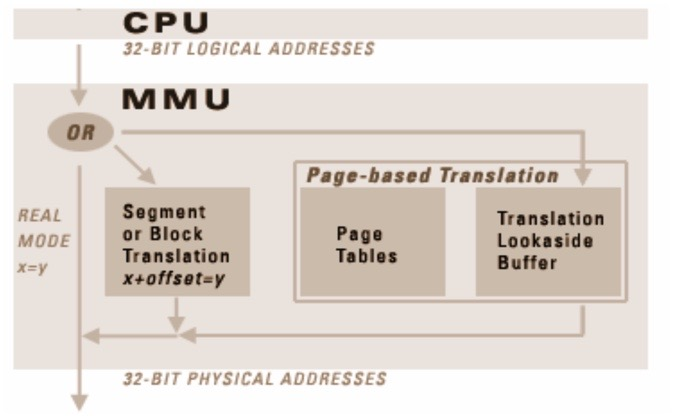
\includegraphics[width=14cm,height=10cm,keepaspectratio]{/Users/daksh_mac/Desktop/mmu.jpeg}
	\caption[About memory]{Memory Management Unit in Lynx OS}
	\label{fig:mmu}	
\end{figure}

\subsection{Memory Allocation Structure}
The Lynx OS download includes five sample memory allocation implementations, each of which are described in the following subsections.

\begin{itemize}
	\item $heap\_1$ - the very simplest, does not permit memory to be freed.
	
	
	\item $heap\_2 $- permits memory to be freed, but does not coalescence adjacent free blocks.
			
	\item $heap\_3 $- simply wraps the standard $malloc()$ and $free()$ for thread safety
	
	\item $heap\_4$ - coalescences adjacent free blocks to avoid fragmentation. Includes absolute address placement option.
	
	\item $heap\_5$ - as per $heap\_4$, with the ability to span the heap across multiple non-adjacent memory areas.


\end{itemize}


\begin{figure}[H]
	\centering
	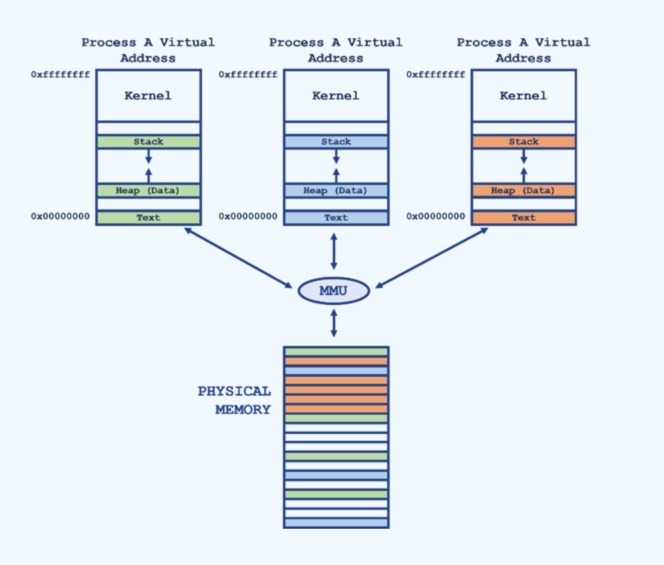
\includegraphics[width=20cm,height=10cm,keepaspectratio]{/Users/daksh_mac/Desktop/mem.jpeg}
	\caption[About memory]{Memory Management in Lynx OS}
	\label{fig:mem}	
\end{figure}


\subsubsection{$heap\_1$}	

$heap\_1$ is the simplest implementation of all. It does not permit memory to be freed once it has been allocated. Despite this, $heap\_1$.c is appropriate for a large number of embedded applications. This is because many small and deeply embedded applications create all the tasks, queues, semaphores, etc. required when the system boots, and then use all of these objects for the lifetime of program (until the application is switched off again, or is rebooted). Nothing ever gets deleted. The implementation simply subdivides a single array into smaller blocks as RAM is requested.\\

The $heap\_1$ implementation:

\begin{itemize}
	\item Can be used if your application never deletes a task, queue, semaphore, mutex, etc. (which actually covers the majority of applications in which Lynx OS gets used).
	
	
	\item Is always deterministic (always takes the same amount of time to execute) and cannot result in \textbf{memory fragmentation}.
		
	\item Is very simple and allocated memory from a statically allocated array, meaning it is often suitable for use in applications that do not permit true dynamic memory allocation.

\end{itemize}	

\subsubsection{$heap\_2$}	

$heap\_2$ uses a \textbf{best fit algorithm} and, unlike scheme 1, allows previously allocated blocks to be freed. It does not combine adjacent free blocks into a single large block\\

The $heap\_2$ implementation:

\begin{itemize}
	\item Can be used even when the application repeatedly deletes tasks, queues, semaphores, mutexes, etc., with the caveat below regarding memory fragmentation.
	
	
	\item Could possible result in memory fragmentation problems if your application queues, tasks, semaphores, mutexes, etc. in an unpredictable order. This would be unlikely for nearly all applications but should be kept in mind.
		
	\item Is not deterministic - but is much more efficient that most standard C library malloc implementations.
	
	\item Should not be used if the memory being allocated and freed is of a random size. For example:
	
	\begin{itemize}
	
		\item[$\circ$] If an application dynamically creates and deletes tasks, and the size of the stack allocated to the tasks being created is always the same, then  $heap\_2$.c can be used in most cases. However, if the size of the stack allocated to the tasks being created was not always the same, then the available free memory might become fragmented into many small blocks, eventually resulting in allocation failures.  $heap\_4$.c would be a better choise in this case.
		
		\item[$\circ$] If an application dynamically creates and deletes queues, and the queue storage area is the same in each case (the queue storage area is the queue item size multiplied by the length of the queue), then  $heap\_2$.c can be used in most cases. However, if the queue storage area were not the same in each case, then the available free memory might become fragmented into many small blocks, eventually resulting in allocation failures.  $heap\_4$.c would be a better choise in this case.
		
	\end{itemize}
	
	

\end{itemize}


\subsubsection{$heap\_3$}	

This implements a simple wrapper for the standard C library malloc() and free() functions that will, in most cases, be supplied with your chosen compiler. The wrapper simply makes the malloc() and free() functions thread safe.\\

The $heap\_3$ implementation:

\begin{itemize}
	\item Requires the linker to setup a heap, and the compiler library to provide malloc() and free() implementations.
	
	
	\item Is not deterministic.
		
	\item Will probably considerably increase the RTOS kernel code size.

\end{itemize}



\subsubsection{$heap\_4$}	

This scheme uses a \textbf{first fit algorithm} and, unlike scheme 2, it does combine adjacent free memory blocks into a single large block (it does include a coalescence algorithm).\\

The $heap\_4$ implementation:

\begin{itemize}
	\item Can be used even when the application repeatedly deletes tasks, queues, semaphores, mutexes, etc..	
	
	\item Is much less likely than the scheme 2 implementation to result in a heap space that is \textbf{badly fragmented} into multiple small blocks - even when the memory being allocated and freed is of random size.
		
	\item Is not deterministic - but is much more efficient that most standard C library malloc implementations.

\end{itemize}		



\subsubsection{$heap\_5$}	

This scheme uses the same first fit and memory coalescence algorithms as scheme 4, and allows the heap to span multiple non adjacent (non-contiguous) memory regions..\\


\subsection{Address Space Protection}

As noted above, LynxOS had a design goal to utilize a processor's page memory
management unit (MMU) to protect each processes logical address space. The MMU also
protects the kernel by placing it in a separate address space.\\
Most competing RTOS products do not offer the flexibility and memory protection
afforded by a complete thread and process model, and rely on unprotected tasks running
in a single flat address space. 
The MMU is used to physically isolate processes from each another so that they cannot
trample on each other's memory. The MMU translates the virtual addresses referenced
by the thread into physical addresses. If a process attempts to address a page that is not
currently mapped to it, the MMU generates an exception.\\
The MMU also allows the process’ memory regions to grow and shrink in order to meet
changing needs of the executing thread. With this, each process has its own protected
address space and can communications between processes through kernel services.




\cleardoublepage

\section{File Management and Secondary Storage}

\subsection{What is a file?}
A file is collection of specific information stored in the memory of computer system.


\subsection{What is file management?}
File management is defined as the process of manipulating files in computer system, it management includes the process of creating, modifying and deleting the files.

\subsection{Role of file management}
The following are some of the tasks performed by file management of operating system of any computer system:

\begin{itemize}
	\item It helps to create new files in computer system and placing them at the specific locations.	
	
	\item It helps in easily and quickly locating these files in computer system.
		
	\item It makes the process of sharing of the files among different users very easy and user friendly.
	
	\item It helps to stores the files in separate folders known as directories. These directories help users to search file quickly or to manage the files according to their types or uses.
	
	\item It helps the user to modify the data of files or to modify the name of the file in the directories.

\end{itemize}	

\subsection{Pillars of File Management}

The file management of function in operating system (OS) is based on the following concepts:

\begin{itemize}
	\item \emph{File Attributes} : It specifies the characteristics of the files such as type, date of last modification, size, location on disk etc. file attributes help the user to understand the value and location of files. File attributes is one most important feature. It is uses to describe all the information regarding particular file.	
	\item \emph{File Operations}: It specifies the task that can be performed on a file such as opening and closing of file.		
	\item \emph{File Access Permission}: It specifies the access permissions related to a file such as read and write.
		
	\item \emph{File Systems} specifies the logical method of file storage in a computer system. Some of the commonly used files systems include FAT and NTFS.
	
\end{itemize}	


Due to paucity of information on all the general important concepts, we are only going to discuss the file system specification in LynxOS.


\subsection{Lynx OS File Systems}

Lynx uses Network File System or Flash File system (embedded structures) for it's specifications	


\subsection{Network File System}

Network File System (NFS) is a distributed file system protocol originally developed by Sun Microsystems (Sun) in 1984, allowing a user on a client computer to access files over a computer network much like local storage is accessed \cite{ref:ten}. NFS, like many other protocols, builds on the Open Network Computing Remote Procedure Call (ONC RPC) system. NFS is an open standard defined in a Request for Comments (RFC), allowing anyone to implement the protocol.


\begin{figure}[H]
	\centering
	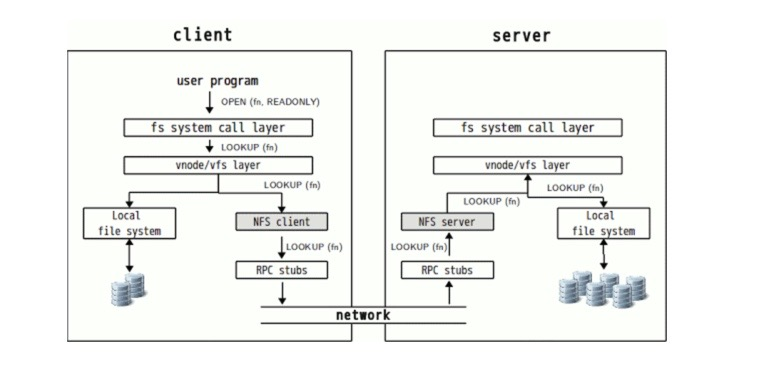
\includegraphics[width=15cm,height=10cm,keepaspectratio]{/Users/daksh_mac/Desktop/nfs.jpeg}
	\caption[About file system]{Network File System Architecture}
	\label{fig:nfs}	
\end{figure}

\subsubsection{NFS Protocol}

\begin{itemize}
	\item Uses Remote Procedure Call (RPC) mechanisms	
	\item RPCs are synchronous (client application blocks while waits for the server response)		
	\item NFS uses a stateless protocol (server do not keep track of past requests) - This simplify crash recovery. All that is needed to resubmit the last request.
	
	\item In this way, the client cannot differentiate between a server that crashed and recovered and one that is just slow.
	

\end{itemize}

\subsubsection{Goals of NFS Design}

\begin{itemize}
	\item \emph{Compatibility} : NFS should provide the same semantics as a local unix file system. Programs should not need or be able to tell whether a file is remote or local. user program: $OPEN("/users/jdoe/.profile", READONLY) -- $program cannot tell whether "users" or "jdoe" are local path names.
	\item \emph{Easy Deployable}: implementation should be easily incorporated into existing systems remote files should be made available for local programs without these having to be modified or relinked.
	\item \emph{Machine and OS Independence}: NFS Clients should run in non-unix platforms Simple protocols that could be easily implemented in other platforms.
		
	\item \emph{Efficiency}: NFS should be good enough to satisfy users, but did not have to be as fast as local FS. Clients and Servers should be able to easily recover from machine crashes and network problems.
	
\end{itemize}	

\subsection{Flash File System}

\subsubsection{Memory Organization}

A NOR flash device memory array is physically divided into sectors or blocks. The File System Component designates them as blocks . Typically, a block's size is 64 kB which is also the smallest erasable unit. Blocks can be further divided, down to memory cells. The memory cell size depends on the device architecture and is 8- (byte), 16 (half word) or 32-bit wide (word). The memory cell architecture also defines smallest programmable unit, which must be maximum 32-bit for use with the Embedded File System.
flash
Embedded File System organizes each block into three regions:

\begin{itemize}
	\item Allocation Information, located on top of the block, grows in descending order and contains file allocation records.
	\item Free Space	
	\item File Names and Content, located on bottom of the block, grows in ascending order and contains file names and data.

\end{itemize}


\begin{figure}[H]
	\centering
	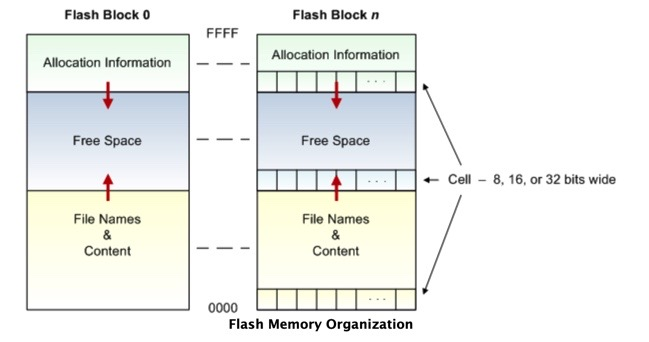
\includegraphics[width=15cm,height=10cm,keepaspectratio]{/Users/daksh_mac/Desktop/flash1.jpeg}
	\caption[About file system]{Flash Memory Organization}
	\label{fig:flash}	
\end{figure}

\subsubsection{Allocation Information}

Allocation information region is located on top of a block and describes the block's content. It consists of block signature and file allocation information records, which are written in descending order. Each file has at least one record associated with it. Multiple records belong to files with content and to fragmented files. A file is fragmented when it is modified or its content size exceeds a single block size and must be stored across several blocks. Several small files are stored into a single block.

\begin{figure}[H]
	\centering
	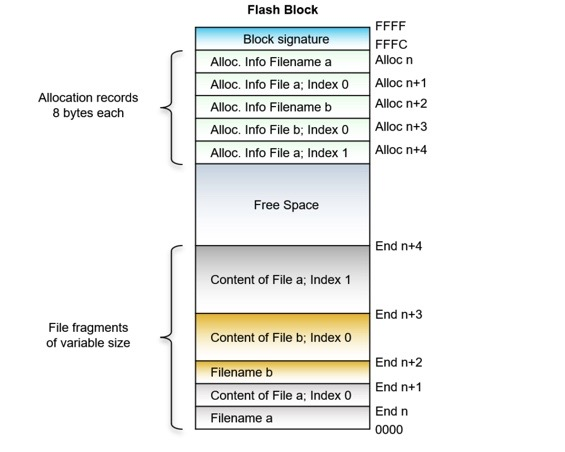
\includegraphics[width=15cm,height=10cm,keepaspectratio]{/Users/daksh_mac/Desktop/flash2.jpeg}
	\caption[About file system]{Flash Block Allocation}
	\label{fig:flash2}	
\end{figure}

\subsubsection{File Names and Content}

The file names and content region is located at the bottom of a block and is fully defined through the file allocation information records. It consists of file names and file content, which can both be fragmented. The first file fragment always starts at the beginning of a block (at offset 0) and is written in ascending order.\\

\textbf{File Names}\\\\
In the Embedded File System, a file name consists of maximum 31 characters. Directories are not supported, therefore any file name which contains a directory separator character, such as slash (/) or backslash, is rejected as invalid. Other characters are allowed.
\cleardoublepage

\textbf{File Content}\\

Since file fragments are of variable size, \textbf{create big file fragments} in order to reduce the total number of file fragments and make the best use of a block. Writing or appending small amounts of data to a file is not optimal, since such an approach creates a large number of allocation information records. They consume free space and the required processing time results in a slow file access time.

When the file content is modified, the old file content is invalidated and a new file fragment is allocated. a block is erased when all the data stored within has been invalidated.

\cleardoublepage

\section{Conclusion}
LynxOS is suitable in embedded systems which contacts with human life like air craft embedded control system .
Lynx OS established four design goals including prompt execution, multithreading,
memory isolation and portability/usability. Development and implmentation of kernel
threads along with priority tracking and utilization of POSIX thread scheduling allows
LynxOS to achieve the first and second goal. The third is achieved through the usage of
MMU and the fourth is fulfilled by the fact that LynxOS was primarily developed using 
C and by adhering to POSIX standards. Together these steps make LynxOS a real time
operating system that is utilized by an impressive list of customers across multiple
industries. 

Here is the our link for the LaTeX source code made for this project: \href{https://github.com/Daksh-404/operating-system-lab/tree/main/mainOSTex}{Source Code}

\cleardoublepage

\bibliographystyle{IEEEtran}
\bibliography{osRef,secondRef,third,fourth,fifth,six,seven,eight,nine,ten,twelve}




\end{document}